% this TeX file provides an awesome example of how TeX will make super 
% awesome tables, at the cost of your of what happens when you try to make a
% table that is very complicated.
% Originally turned in for Dr. Nico's Security Class
\documentclass[11pt]{article}


% Use wide margins, but not quite so wide as fullpage.sty
\marginparwidth 0.5in 
\oddsidemargin 0.25in 
\evensidemargin 0.25in 
\marginparsep 0.25in
\topmargin 0.25in 
\textwidth 6in \textheight 8 in
% That's about enough definitions
\usepackage{listings}

% multirow allows you to combine rows in columns
\usepackage{multirow}
% tabularx allows manual tweaking of column width
\usepackage{tabularx}
% longtable does better format for tables that span pages
\usepackage{longtable}
\usepackage{graphicx} %package to manage images
\graphicspath{ {images/} }
\begin{document}
% this is an alternate method of creating a title
%\hfill\vbox{\hbox{Gius, Mark}
%       \hbox{Cpe 456, Section 01}  
%       \hbox{Lab 1}    
%       \hbox{\today}}\par
%
%\bigskip
%\centerline{\Large\bf Lab 1: Security Audit}\par
%\bigskip
\author{Daniel Ocampo}
\title{Lab 3: Introduction to R.}
\maketitle

\section{Objectives}
\begin{itemize}

\item To enhance the understanding of the basic R functionality, including the use of R Studio and producing data visualizations. 
\item Reading Assignment: Chapters 3, 4, 6 and 8 

\end{itemize}

\section{Questions}
The questions to answer are the following.
{3.2.4, 3.3.1, 3.5.1, 3.6.1, 3.7.1, 3.8.1, 3.9.1, 4.4, 6.3}
Note: For the question 6.3.1, where a tip is adopted from Twitter, please give the tip and then explain how it is useful to you.

% defines a table that spans pages with columns defined by the sizes seen here
% see http://en.wikibooks.org/wiki/LaTeX/Tables for more information, especially
% sections on spanning and resizing tables

\section{ Chapter 3 from textbook}

\begin{lstlisting}[language=R]
       install.packages("tidyverse")
    library(tidyverse)
    package::function()
    ggplot2::ggplot()
    ggplot2::mpg
    ?mpg
    ggplot(data = mpg) + 
      geom_point(mapping = aes(x = displ, y = hwy))
#ploting     
    ggplot(data = mpg)
#making the data equal to mpg

    ggplot(data = mpg) + 
      geom_point(mapping = aes(x = cyl, y = hwy))
    # cylinder to miles in highway
    ggplot(data = mpg) + 
      geom_point(mapping = aes(x = class, y = drv))
      #the type to  wheel drive
      ggplot(data = mpg) + 
  geom_point(mapping = aes(x = displ, y = hwy, color = class))
      #changing the color by type E.g 
      ggplot(data = mpg) + 
        geom_point(mapping = aes(x = displ, y = hwy, size = class))
      #changing the size of the display
      ggplot(data = mpg) + 
        geom_point(mapping = aes(x = displ, y = hwy, alpha = class))
      #changing by shading 
      ggplot(data = mpg) + 
        geom_point(mapping = aes(x = displ, y = hwy, shape = class))
      #difftent shape to type of car
      ggplot(data = mpg) + 
        geom_point(mapping = aes(x = displ, y = hwy), color = "blue")
      #change data to all blue 
      
      ggplot(data = mpg) + 
        geom_point(mapping = aes(x = displ, y = hwy, color = "blue"))
      mpg##
      View(mpg)
      ## displays all of the data 
      #next three will be about 3.3.1 question 3 
      ggplot(data = mpg) +
        geom_point(mapping = aes(x = displ, y = hwy, color = cty)) 
      ### making some R code with continous values for color 
      ggplot(data = mpg)+
        geom_point(mapping = aes(x = displ , y = hwy , shape = class))
      ### making shapes based off class
      ggplot(data = mpg)+
          geom_point(mapping = aes(x = displ , y = hwy , size = trans))
      ### the size of the plots based on the transmission 
      #### 3.3.1 Question 4 
      ggplot(data = mpg)+
        geom_point(mapping = aes(x = displ , y = hwy , size = trans, color = trans))
      ## what if we add mutliple arguments we can get a mixture of both 
      ?geom_point
      ## for help Use the stroke aesthetic to modify the width of the 
      # border 
      ggplot(mtcars, aes(wt, mpg)) +
        geom_point(shape = 21, colour = "black", fill = "white", size = 5, stroke = 5)
      #exa  mple from ?geom_point
      
      ggplot(data = mpg) + 
        geom_point(mapping = aes(x = displ, y = hwy)) + 
        facet_wrap(~ class, nrow = 2)
      #### seprating data based on class 
      ggplot(data = mpg) + 
        geom_point(mapping = aes(x = displ, y = hwy)) + 
        facet_grid(drv ~ cyl)
      ### plot a grid   
\end{lstlisting}

\newpage
\noindent\textbf{3.2.4 Exercises}


\begin{enumerate}
    


\item Run ggplot(data = mpg). What do you see?\\
\textbf{I did not see anything when the code ran.} 
\item How many rows are in mpg? How many columns?\\
\textbf{I would say that there is 0 rows for mpg and two columns for MPG, both hwy and cty. (The view of the data is down below).}
\begin{figure}[t]
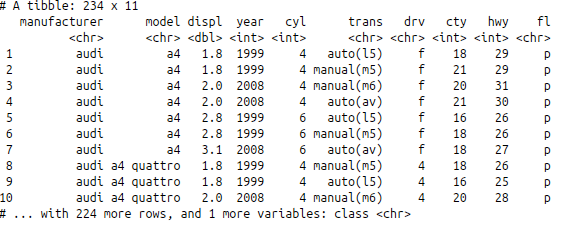
\includegraphics[scale = .5]{chart.png}
\centering
\end{figure}

    
\item What does the drv variable describe? Read the help for ?mpg to find out.\\
\textbf{F = Front-wheel drive \\
4 = Four wheel drive  \\ 
R = Rear wheel drive 
}


\item Make a scatterplot of hwy vs cyl.
\begin{lstlisting}[language=R]
 ggplot(data = mpg) + 
      geom_point(mapping = aes(x = cyl, y = hwy))

\end{lstlisting}
The output is posted in the figure below. 
\begin{figure}[h]
\includegraphics[scale = .25]{cyl:hwy.png}
\centering
\end{figure}


\item What happens if you make a scatterplot of class vs drv? Why is the plot not useful?
\begin{lstlisting}[language=R]
 ggplot(data = mpg) + 
      geom_point(mapping = aes(x = class, y = drv))
\end{lstlisting}



\textbf{It has no useful information, what point of knowing what brand they are and if it is rear or 4 wheel drive, not important information. (The image below shows the output of the code). }

\begin{figure}[ht]
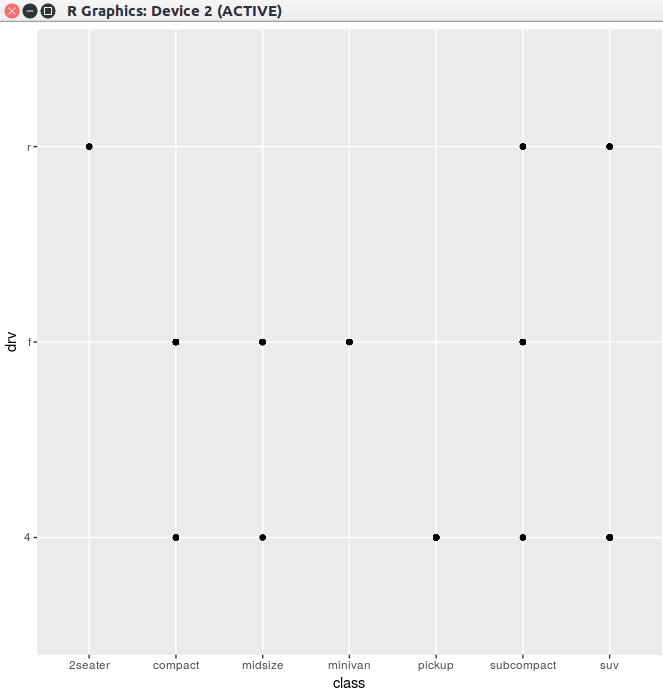
\includegraphics[scale = .25]{drv.png}
\centering
\end{figure}
\end{enumerate}


\newpage

\noindent\textbf{3.3.1}
\begin{enumerate}
    \item What’s gone wrong with this code? Why are the points not blue?\\ \textbf{The reason why it is not blue is because it needs to go out the aesthetic
    }
    
\begin{figure}[h]
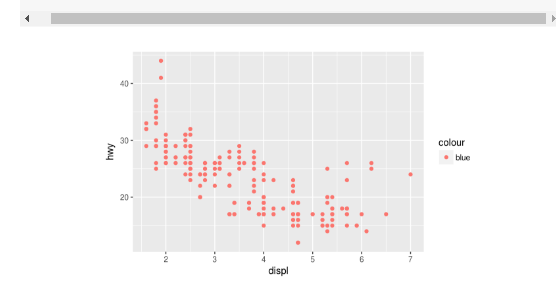
\includegraphics[scale = .7]{sample.png}
\centering
\end{figure}
    \item Which variables in mpg are categorical? Which variables are continuous? (Hint: type ?mpg to read the documentation for the dataset). How can you see this information when you run mpg?
    
  \textbf{I would say that model, manufacturer, trans, drv, class would be considered categorical. Variables that are considered continuous would be city, hwy ,cyl, and displ. when I type in mpg, I get to see what are int and strings, so it can give me a better guess of weather it is categorical or continuous. }
  
  \item Map a continuous variable to color, size, and shape. How do these aesthetics behave differently for categorical vs. continuous variables?
  \begin{lstlisting}[language=R]
    #next three will be about 3.3.1 question
    ggplot(data = mpg) +
        geom_point(mapping = aes(x = displ, y = hwy, color = cty)) 
     ### making some R code with continous values for color 
      ggplot(data = mpg)+
        geom_point(mapping = aes(x = displ , y = hwy , shape = class))
      ### making shapes based off class
      ggplot(data = mpg)+
          geom_point(mapping = aes(x = displ , y = hwy , size = trans))
      
       \end{lstlisting}
       \newpage
    \item What happens if you map the same variable to multiple aesthetics? 
    
    \begin{lstlisting}[language=R]
     ggplot(data = mpg)+
     geom_point(mapping = aes(x = displ , y = hwy , size = trans,
     color = trans))
    \end{lstlisting}
      \textbf{The thing that you get is a mixture of both of them, so you would get the size and the color at the same time. }
      
      \item What does the stroke aesthetic do? What shapes does it work with? (Hint: use ?geom\_point)
      
      \textbf{According R studio, it Uses the stroke aesthetic is to modify the width of the border.}
      o
      \begin{lstlisting}[language=R]
       ggplot(mtcars, aes(wt, mpg)) +
  geom_point(shape = 21, colour = "black", fill = "white", size = 5, 
  stroke = 5)

      \end{lstlisting}
      
\textbf{This was the example that was given, so apparently it supports size.}    

\item What happens if you map an aesthetic to something other than a variable name, like aes(colour = displ < 5)?

\textbf{
Well I think what is going to happen is that it going to give a true or false, and change the colors based on part of the spectrum the engine size is located.}
      \end{enumerate}
     \newpage
     
     
\noindent\textbf{ 3.5.1}     
      
      
      \begin{enumerate}
          \item What happens if you facet on a continuous variable?\\
          \textbf{well continuous data may be to much for R studio, it would be hard to plot continuous data. In my opnion it would be point less because what if you have a data point by itself in a graph }
          
          
          \item What do the empty cells in plot with facet\_grid(drv
          ~ cyl) mean? How do they relate to this plot?
          
         \begin{lstlisting}[language=R]
         ggplot(data = mpg) + 
  geom_point(mapping = aes(x = drv, y = cyl))
          
         \end{lstlisting}
         
          \textbf{  The following code just has few points showing that there are cars with front wheel drives, have 4 cylinders and so on so fourth, Don't see how this data can be useful. 
        }

        \item What plots does the following code make? What does . do?\\
     \textbf{The . function is similar to ~ in that it is used to capture the name of variables, not their current value. This is used throughout plyr to specify the names of variables (or more complicated expressions).}


         \begin{lstlisting}[language=R]
         
         ggplot(data = mpg) + 
  geom_point(mapping = aes(x = displ, y = hwy)) +
  facet_grid(drv ~ .)

         \end{lstlisting}
         
         
        \textbf{ This part of code make a longer horizontal grid which, just puts all of the types on grid and plot miless on hwy based on how big the size of the engine while also separating them by the wheel drive.  }
        
        
         \begin{lstlisting}[language=R]
         
         ggplot(data = mpg) + 
  geom_point(mapping = aes(x = displ, y = hwy)) +
  facet_grid(cyl~ .)

         \end{lstlisting}
\textbf{The same thing but just based on the cylinders.}


\item Take the first faceted plot in this section:

  \begin{lstlisting}[language=R]
         
         ggplot(data = mpg) + 
  geom_point(mapping = aes(x = displ, y = hwy)) +
  facet_grid(drv ~ .)

         \end{lstlisting}
         
What are the advantages to using faceting instead of the colour aesthetic? What are the disadvantages? How might the balance change if you had a larger dataset?

Well this is a hard question to answer because, it all depends on the dataset 



      \end{enumerate}
      \newpage
      
\noindent\textbf{3.6.1}
      
     \begin{enumerate}
         \item What geom would you use to draw a line chart? A boxplot? A histogram? An area chart? \\
\textbf{I can figure this problem out by simply doing the ?ggplot.\\ 
 geom\_line() = a line chart\\ 
 geom\_boxplot()= box plot chart\\ 
geom\_histogram() = a historgram box\\
geom\_area()= this equalts a area chart.} 

\item Run this code in your head and predict what the output will look like. Then, run the code in R and check your predictions.

\begin{lstlisting}[language= R]
 ggplot(data = mpg, mapping = aes(x =
 displ, y = hwy, color = drv)) + 
  geom_point() + 
  geom_smooth(se = FALSE)
    
\end{lstlisting}

\textbf{I think the graph is going to produce the engine size compared to amount of miles, while changing the color by the wheel drive.} \\

\textbf{What happened when I ran this is exactly what I thought would happen the only difference is that I forgot to mention the smooth part, which would draw a line. around the areas where wheel drive had switched. 
}

\item What does show.legend = FALSE do? What happens if you remove it?
Why do you think I used it earlier in the chapter?\\

\textbf{It removes the legend, I think he used to help show how to make line of a scatter plot. }

\item What does the se argument to geom\_smooth() do.

\textbf{I think what it does is a condtion so if it true draw the line else if do not draw it. }

\item Will these two graphs look different? Why/why not?

\begin{lstlisting}{language = R}
 ggplot(data = mpg, mapping = 
 aes(x = displ, y = hwy)) + 
  geom_point() + 
  geom_smooth()

ggplot() + 
  geom_point(data = mpg, mapping =
  aes(x = displ, y = hwy)) + 
  geom_smooth(data = mpg, mapping =
  aes(x = displ, y = hwy))

\end{lstlisting}


\textbf{
I am not sure because they use the same data, It should produce the same graph, but there is a lot details that might be missed in the format of the code }
         
         
   
      
  \item Recreate the R code necessary to generate the following graphs.    
  \begin{figure}[h!]
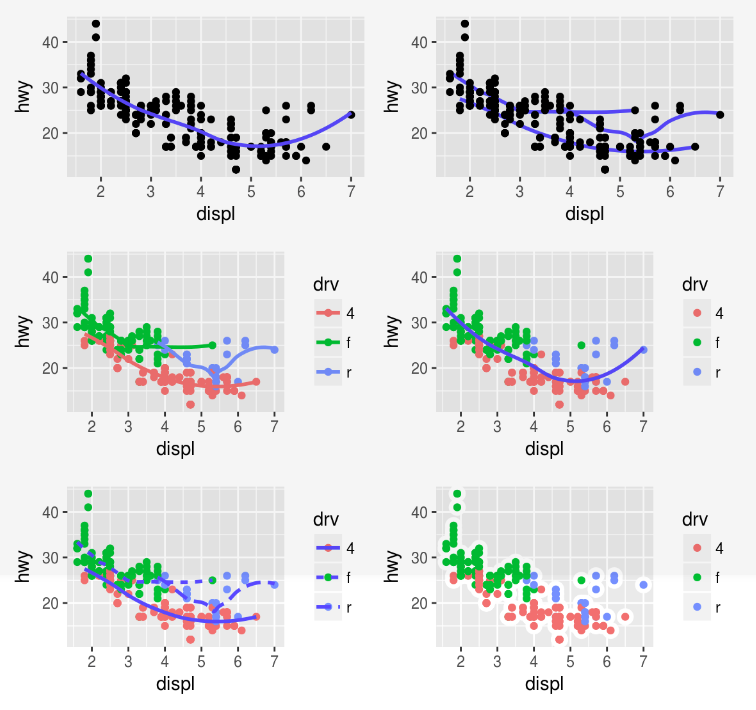
\includegraphics[scale = .5]{recreategraphs.png}
\centering
\end{figure}
    
  \begin{lstlisting}{language = R}
   ggplot(data = mpg, mapping = aes(x = displ, y = hwy)) + 
  geom_point() + 
  geom_smooth(se = FALSE)
  ##### number 1
  ggplot(data = mpg, mapping = aes(x = displ, y = hwy)) + 
  geom_smooth(aes(group = drv), se = FALSE) +
  geom_point()
  #### number 2
  ggplot(data = mpg, mapping = aes(x = displ, y = hwy, color = drv)) + 
  geom_point() + 
  geom_smooth(se = FALSE)
  
  ### number 3
  
  ggplot(data = mpg, mapping = aes(x = displ, y = hwy)) + 
  geom_point(aes(color = drv)) + 
  geom_smooth(se = FALSE)
  
  ### 4 
  ggplot(data = mpg, mapping = aes(x = displ, y = hwy)) + 
  geom_point(aes(color = drv)) +
  geom_smooth(aes(linetype = drv), se = FALSE)
  
  ### number 5
  ggplot(data = mpg, mapping = aes(x = displ, y = hwy)) + 
  geom_point(size = 4, colour = "white") + 
  geom_point(aes(colour = drv))
  
  ### number 6
  
  
  \end{lstlisting}    
      
  \end{enumerate}
  
  
 \noindent\textbf{3.7.1} 
 \begin{enumerate}
 \item What is the default geom associated with stat\_summary()? How could you rewrite the previous plot to use that geom function instead of the stat function?
 
 \end{enumerate}
  
  
          







\end{document}
